

\documentclass{article}
\usepackage{graphicx}
\graphicspath{  }

\begin{document}
\begin{center}

  \title{Figuras, solucion de la ecuacion de onda}
\date{Noviembre 11, 2017}
\author{Mario C.\\ 201512863, Universidad de los Andes}
\maketitle
  
  \begin{figure}[t]
    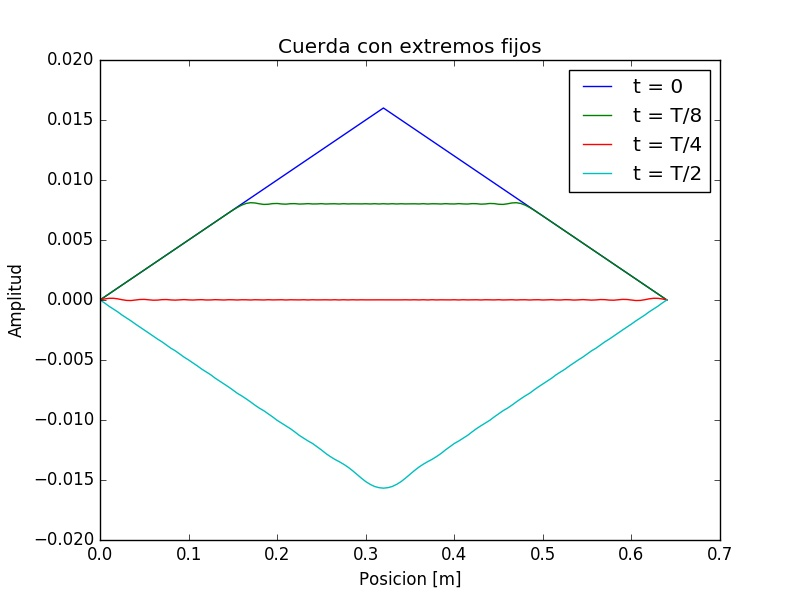
\includegraphics[width=\textwidth]{extremos_fijos}
    \centering
    \\
    En esta imagen se observa la solucion numerica de una cuerda con extremos fijos y una condicion inicial dada. La solucion se presenta en distintos instantes de tiempo (t = 0, T/8, T/4 y T/2).
  \end{figure}
  

  \begin{figure}[t]
    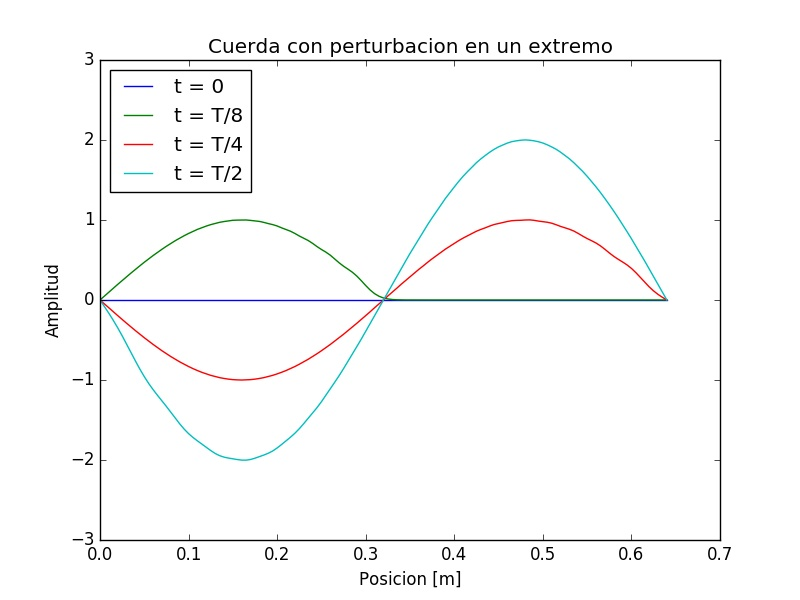
\includegraphics[width=\textwidth]{extremos_perturbacion}
    \centering
    \\
     En esta imagen se observa la solucion numerica de una cuerda con un extremo fijo y un extremo libre con perturbacion sinusoidal. La solucion se presenta en distintos instantes de tiempo (t = 0, T/8, T/4 y T/2).
  \end{figure}

  \begin{figure}[t]
    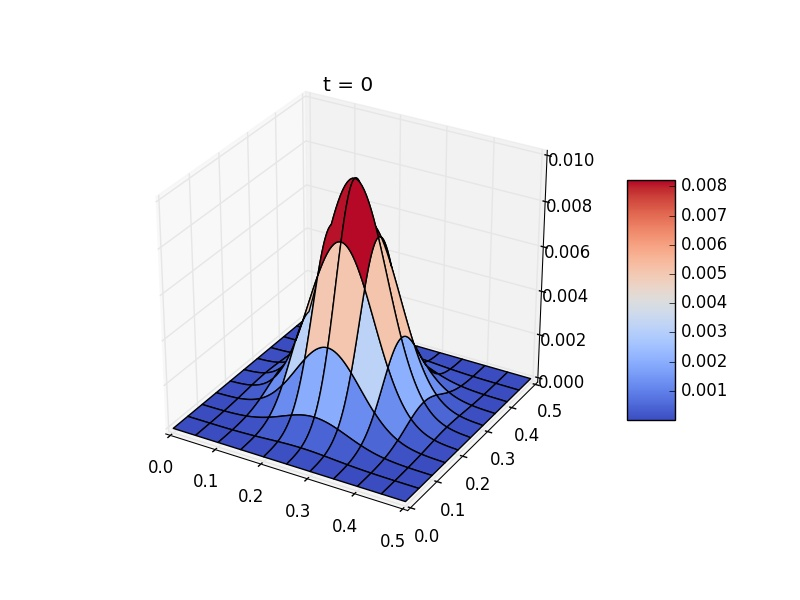
\includegraphics[width=\textwidth]{tambor_t0}
    \centering
    \\
    Perturbacion en el tambor cuadrado para t = 0 (cond. inicial).
  \end{figure}

  \begin{figure}[t]
    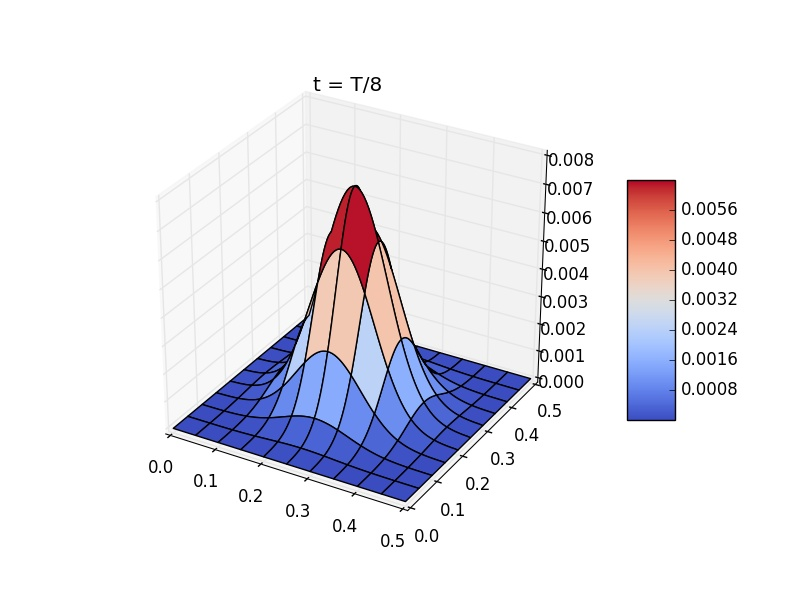
\includegraphics[width=\textwidth]{tambor_t8}
    \centering
    \\
    Perturbacion en el tambor cuadrado para t = T/8.
  \end{figure}

  \begin{figure}[t]
    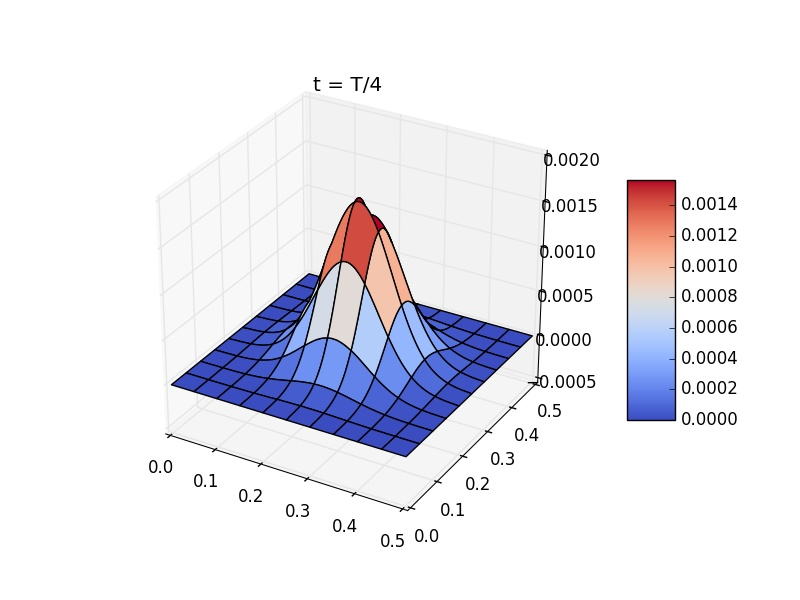
\includegraphics[width=\textwidth]{tambor_t4}
    \centering
    \\
    Perturbacion en el tambor cuadrado para t = T/4.
  \end{figure}

  \begin{figure}[t]
    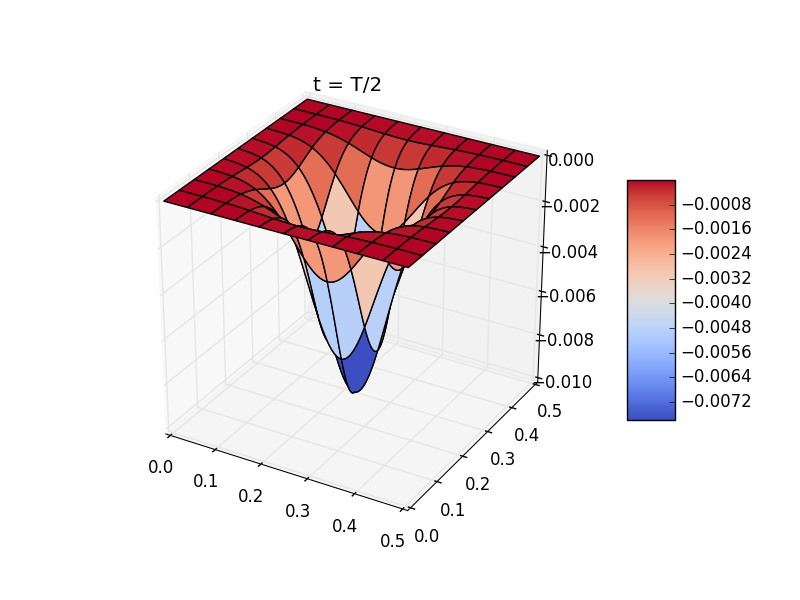
\includegraphics[width=\textwidth]{tambor_t2}
    \centering
    \\
    Perturbacion en el tambor cuadrado para t = T/2.
  \end{figure}
 
 
\end{center}


\end{document}

